\chapter{P2P MMVE state management and persistency}
\label{p2p_MMVE_state_persistency}
%%%%%%%%%%%%%%%%%%%%%%%%%%%%%%%%%%%%%%%%%%%%%%%%%%%%%%%%%%%%%%%%%%%%%%%

While the previous chapter broadly introduced all the concepts of state consistency, this chapter will focus solely on state management and state persistency in P2P MMVEs. State management and persistency in P2P MMVEs respectively allow for the short- and long term storage of game data. The fact that game data are now distributed amongst various peers in the network creates challenges not usually present in classic C/S MMVEs.

This chapter classifies the techniques used in documented P2P MMVE architectures and discusses the advantages and disadvantages of the different types of storage. The chapter also shows that no current storage type is well suited to P2P MMVEs.

\section{A definition of state management and state persistency}
\label{management_persistency_def}

A discussion of state storage requires an understanding of the difference between state management and state persistency. These terms are regularly confused in the literature and sometimes one is used where the other is more appropriate. Authors describe both mechanisms as if it is all part of the same model.

Storing authoritative data requires state management and state persistency. State management is the storage of objects in primary storage, while state persistency is the storage of the VE on secondary storage. State persistency does not have such rigorous responsiveness requirements as state management, as explained in Section \ref{char_responsiveness}.

In this work, state persistency is defined to mean long term data storage. This means that if a server or client goes off-line, the state persistency mechanism will ensure the safe storage of the state for when the server or client starts up again. State persistency is, therefore, storage in secondary persistent memory. All servers require state persistency to back-up the VE state in case of some outage or in case a server restart is required. This storage type does not require low latency, but needs to be reliable. State persistency in P2P MMVEs is therefore taken to mean the same. It does not have to be fast, but when a client logs out of the VE and logs back in again, the stored state should remain.

State management is defined to mean the storage of the VE state in primary memory. This is the state with which the server and clients will interact. It is the state that will be displayed to the agent on the client and it is the state that will require fast retrieval and storage as a result of received events or updates. State management is used to:
\begin{enumerate}
\item apply generated or received object updates to authoritative objects on the authoritative node,
\item apply received object updates to non-authoritative objects on non-authoritative nodes, and to
\item supply information of other objects needed by the environment logic, in order to generate authoritative object updates for a received event.
\end{enumerate}

Although state management and state persistency are two different types of storage, with different storage requirements, there are also similar aspects between state management and persistency. Since state management and persistency are very similar (as discussed in Section \ref{key_challenges_cm}), the term ``storage'' will be used when referring to both.

Many ``storage types'', which can be used for either state management or persistency are discussed in this chapter. The reference of the storage type to state management and/or persistency will be discussed where applicable.

Before discussing storage techniques that have been developed for P2P networks, a review of classic state management and persistency architectures used in C/S based systems will be reviewed.

\section{Client/Multi-Server state management and persistency models}
\label{cms_models}

This section introduces the classic state management and persistency architectures used in server cluster or client/muli-server based systems \cite{Hu_voronoi_IM}.

\subsection{Sharding}
\label{sharding}

A storage model where the VE state is duplicated over multiple servers, with players connecting to one of these servers is termed ``sharding''. For all practical purposes, this approach is still merely a C/S approach, with players forced into a specific C/S environment. Each shard hosts the global authoritative state and thus state management and persistency is performed centrally by the shard server, where all objects are stored.

\subsubsection{Advantages}

Sharding has the following advantages:
\begin{itemize}

\item It allows for greater scalability than the single server approach, since the maximum load is fixed and more shards can be added as the environment becomes popular.

\item It is relatively simple to implement, because no inter-server communication is required and no server migration is supported.

\item It allows for a relatively small environment to support many players because of the duplication of the worlds. This reduces the load on level designers and content designers, who now have to populate a much smaller world with content.
\end{itemize}

\subsubsection{Disadvantages}

Sharding has the following disadvantages:
\begin{itemize}
\item Clients are not able to interact or communicate with players on other shards, which reduces game immersion.

\item Players are not able to enter a shard if that shard has reached its capacity. In the past, this has caused unhappiness amongst players, since popular shards could be difficult to log in to. Players are also reluctant to move to a new shard, because a lot of time is invested in their characters in their ``home'' shard.

\item Inefficient resource allocation occurs, as one shard may be overpopulated while another is underpopulated.
\end{itemize}

\subsection{Replication-based}
%Redundant
The replication-based model is similar to sharding, with the difference that all servers share the same duplicated game state. Each server contains the global game state and clients connect to any one of these servers (mirror-servers \cite{mirrored_server}) or through a load distribution algorithm to a server (proxy-servers \cite{proxy_server_dist}).
Each server handles all actions from clients and updates its own database. The servers in turn send updates to each other over a high quality link, such as fibre, to maintain database consistency at high speeds.

\subsubsection{Advantages}

The replication-based scheme improved upon sharding in that users are now part of the same virtual world. In order to enable the virtual world to host more players, more servers may be added.

\subsubsection{Disadvantages}

The problem with this system is that two users standing next to each other in the virtual world, might be on different servers and, therefore, experience two slightly different worlds. Players are more likely to interact with other player who are close to them, than players who are far away. For this interaction to occur, the messages might now have to traverse servers. Sending a message to another server is a much more expensive operation than transferring information between two users within the same server. This required a message to be sent to another server, as opposed to an internal signal within the same server.

The single shared database still limits the number of concurrent players that can connect to the world.

\subsection{Zone or region-based}
%Zone-based
The zone-based (also called region-based) storage model divides the virtual world into zones or regions, which are hosted on different servers \cite{zone_based_stat}, \cite{zone_based_dyn}. Region-based models can be divided into static region and dynamic region approaches. In static region approaches busy regions are hosted on their own servers, while multiple quiet regions are hosted on a single server. Dynamic regions are being investigated, where regions can be dynamically shifted from one server to another, in order to balance load \cite{zone_based_dyn}.

\subsubsection{Advantages}

The advantage of region-based state management is that all players who are close to each other are likely to be hosted on the same server. Users interaction on the same server are more responsive and require less overhead than user interactions between servers.

\subsubsection{Disadvantages}

The disadvantage of the static region approach is that it does not scale well when one region is suddenly populated with users. This type of behaviour happens quite regularly and is known as flocking \cite{flocking}. When players find something of interest in a region, many players will flock to that region. The solution to flocking has been over provisioning of resources to handle peak loads. When peak loads do not occur, the over provisioned hardware is, however, wasted.

If servers become overloaded, while others have resources to spare, some servers may have to be brought off-line to balance region load amongst the over-loaded and under-loaded servers. This will cause the VE to be unavailable during that time.

Dynamic regioning solves the issues related to flocking and transient loads, but this approach adds overhead and significant complexity with regards to the migration of the data and the handling of player actions while the data are in transit. No current, commercially successful, VE is known to make use of dynamic regioning.

\subsection{Object-based}

The object-based storage model equally distributes all in-game objects amongst the servers \cite{object_based_consistency1}, \cite{object_based_consistency2}, \cite{object_based_consistency3}. For an MMVE, most of these objects are expected to be player objects.

\subsubsection{Advantages}

The advantage of this method is that the system load is fixed for a certain player population and that the load is equally distributed amongst all servers. This allows for more accurate prediction and provisioning of resources, but still does not handle transient loads well.

\subsubsection{Disadvantages}

The inter-server communications are random and also more than the inter-server communications for a region based system. The reason for this is that the number of player interactions increase with a decrease in the distance
between the players. Players playing together move together, chat and interact with NPCs together. For a region based model, all player-neighbour interactions remain local to the server.

\subsection{Conclusion}

Examining the disadvantages and advantages of each classic storage method, the two methods that seem most promising are the region-based and object-based approaches. Sharding doesn't allow for a single world or any form of load balancing and replication-based schemes still have the single database as a bottleneck.

Because of the advantages of region-based storage, it has become a popular storage architecture to employ for online worlds. Most worlds can be divided into regions and the game world can be designed in such a way that region boundaries are difficult to cross and that users can only cross these boundaries when moving from one distinct area into the next. This can be done by placing high mountain ranges on region boundaries, with a single pass through the range. This prevents users from switching between regions if they stand on a region boundary. It also ensures that most users that interact, do so within the same server, which decreases inter-server communication.

An issue with the region-based approach, compared to the object-based approach is that each region contains many users and, therefore, requires a large server to host a region. Some region-based servers are themselves server clusters to handle the client load. An object-based server on the other has a fixed load, which can be determined based on the number of objects each server stores.
Because of the success of the object-based and region-based storage schemes, P2P storage schemes are also based on either of the two. Because peers are less powerful than servers, the object-based approach seems to have gained more traction, since server load is fixed. If a region-based approach is used, peers are required to host large regions, which might overload them. If a the region is made too small, the amount of inter-peer communication might become prohibitive.

\section{P2P MMVE storage requirements}
\label{key_challenges_cm}

In order to evaluate the suitability of the existing P2P MMVE storage architectures we will first identify and define a number of requirements for storage. These requirements are based on the reviewed literature and is a combination of the various issues that each of the existing architectures identified. In the following section we will review the existing architecture using the metrics defined in this section and show that no one architecture meets all the requirements.

%Consistency issues
The key challenges related to P2P MMVE storage models are: fairness, overhead, reliability, responsiveness, scalability and security. All storage models will be reviewed with these characteristics in mind. The identified metrics allow for different storage models to be compared and provide a measure of the applicability of any storage model to P2P MMVEs.

\subsection{Scalability}
\label{scalability_req}
Scalability underpins all evaluation criteria. This implies that for a system to be scalable, all other evaluation criteria should be satisfied for large numbers of peers and data. For this reason, scalability will not be explicitly reviewed in the following storage types. Rather, all other evaluation criteria will be evaluated for a large number of peers, thereby taking into account scalability.

The question of what constitutes a large number of peers arises. To establish what an adequate number of peers is, current MMVE architectures can be used for inspiration. \emph{It is proposed that to classify a system as sufficiently scalable, 2500 peers is the smallest number of peers that a system must accommodate}. This is the number of players per server (realm), currently supported by most active C/S MMVEs. For a system to be classified as \emph{truly scalable}, it is believed that the architecture should support 60,000 concurrent users, twenty times more than a sufficiently scalable system. This is the number of peak concurrent users (PCUs) currently supported by the super computer used to host Eve Online \cite{eve_pcu}. These two measures will ensure that a system is as scalable as other currently available architectures.

For systems that will support the MMVEs of the future, it is believed that a target of 1 million peers should be used. This number is sixteen times that of a truly scalable system and the peak concurrent player count of World of Warcraft in China in 2008 \cite{WoW_china_pcu}. Systems that will support these numbers can be classified as \emph{highly scalable}. It is important to note that no current systems support such a large PCU count on a single server cluster. The PCU count presented for WoW is the PCU count over all server clusters hosting WoW in China \cite{WoW_china_pcu}.

\subsection{Fairness}
\label{fairness_requirement}

Ensuring fairness in the system means distributing load evenly according to the abilities of individual nodes. This ensures that not only a small number of nodes provide all system resources required for the system to function, but that all nodes contribute what they can, in order to support the system.

Fairness does not exclude heterogeneity of nodes. It is accepted that nodes have different amounts of available resources. It also does not exclude node specialisation. It is accepted that some P2P architectures require specialised nodes or require a set of different types of super peers to function. Fairness merely states that when all node contributions are added, the sum of all node contributions should be equal.

\emph{Fairness can be evaluated by evaluating the distribution of game state amongst all nodes in the P2P network.} This can be measured at a file level, i.e. what is the standard deviation of the number of files contained on each node, or on byte level, i.e. what is the standard deviation of the number of bytes stored on each node. A lower standard deviation will point to a fairer data storage scheme, if it is assumed that all nodes should contribute an equal amount of storage.

\subsection{Reliability}

For the storage to be reliable, it must be impossible for data to be lost, and stored data should always be available when a node requests it. Reliability encompasses both robustness and availability. Robustness means that the data should be resilient to network churn and availability means that data should be available to any node in the network, if the node has permission to access the data.

\emph{Reliability can be measured as the percentage of successful storage and retrieval requests, compared to the total number of storage and retrieval requests.}

\subsection{Responsiveness}
\label{char_responsiveness}

Responsiveness is the only requirement that is of lower priority for state persistency, compared to state management. Since it is assumed that all low-latency data requests will be handled by state management, state persistency is only used to archive environment state, and thus responsiveness is less of a priority. Highly responsive state persistency will still improve data throughput and ensure that less data will be lost in the event of a failure, but highly responsive state management is required for the correct functioning of the state consistency mechanism.

To ensure system responsiveness, objects must be stored or retrieved in real-time. With real-time, it is meant that data should be available within a certain time frame that would ensure correct functionality of the MMVE requiring it. For classic MMORPGs, acceptable latency is anything under a second \cite{WoW_delay_effect}, but preferably under 500ms. The variance in data retrieval times should be small. \emph{Responsiveness can be measured by the time it takes to read or write data to the storage network.}

\subsection{Security}
\label{characteristics_security}

The storage system should store data securely. It should not be possible for data to be altered in ways that are inconsistent with the environment logic. It should also be possible to identify nodes that alter the data in a malicious way. This also adds the requirement that nodes should be authenticated in the storage system and that only authorised nodes should be able to alter data. According to \cite{distributed_systems_security}, security is the combination of a number of objectives: Authentication, Authorisation, Data Integrity, Confidentiality, Availability, Trust, Privacy and Identity Management.

For a storage model to address the above mentioned security objectives, a certification scheme with public and private key encryption is required. Such a scheme allows for the identification of users, and by having users sign any storage interactions, every change made to the storage system can be tracked. This is a major differentiating factor from classic distributed storage systems such as Freenet, where a primary objective is anonymity. If all operations are logged and all users have to be identifiable for a secure system, no user can be anonymous.

It is difficult to define a single measurement criteria for security. In this work we take the same approach as the approach taken with scalability. Where the scalability criteria specifies that all requirements should be met for large numbers of nodes, the security criteria is defined to specify that all requirements should be met for various percentages of malicious nodes present in the network. \emph{In other words, security specifies that the system should remain reliable, responsive and fair for various percentages of malicious users in the network.}

\subsection{Overhead}
\label{characteristics_overhead}

The amount of bandwidth required by the storage system, compared to the amount of objet data stored, should be low. Any networked communications protocol should attempt to limit its overhead. A system with low overhead has a faster effective data transfer rate, compared to a system with high overhead if the same bandwidth is available.

\emph{For a given storage type, or any network layer, overhead can be measured as the factor of data received from or delivered to the higher layer, compared to the bandwidth required to handle the higher layer requests in the storage layer.}

For the storage systems discussed below, little empirical evidence is available as to the overhead that the various systems require. Overhead is also directly proportional to the number of redundancy in the storage systems, i.e. the number of replicas used. This is usually a configuration parameter of the storage system and it is difficult to judge what the required number of object replicas are to achieve desired levels of reliability. Due to these issues, overhead will not be reviewed in this literature study. Overhead will, however, be evaluated when our own storage system is evaluated in Chapter \ref{chp:EVALUATION}, and the overhead measured will be compared with the overhead of a currently implemented storage system (overlay storage, as discussed in Section \ref{overlay_storage}).

\section{Overview of P2P MMVE storage types}
\label{storage_type_overview}

In this section four approaches to state persistency in P2P MMVEs is discussed: \emph{super peer storage}, \emph{overlay storage}, \emph{distance-based storage} and \emph{hybrid storage}. Each storage type is evaluated in terms of the requirements identified in Section \ref{key_challenges_cm}.

%Centralised storage
Two other types of storage sometimes described in P2P MMVEs papers are \emph{centralised storage} and \emph{individual storage}. Centralised storage is storage in a centralised database, the same as for a C/S MMVE \cite{badumna_engine}, \cite{rooney_centralised_storage}, \cite{hybrid_p2p_cs_centralised}. Centralised storage for an MMVE requires the same large expensive servers and high bandwidth as required by a classic C/S architecture and therefore does not fit into the P2P MMVE paradigm. For this reason, centralised storage will not be evaluated in this chapter.

%Individual storage
With individual storage, player data are stored on a player's own computer  \cite{individual_storage1}, \cite{cheat_proof_playout}. These architectures do not address the storage of NPC state or mutable objects. These objects cannot be as easily mapped to a single peer in the network as player state can and, therefore, require a mapping mechanism to decide where to host these objects. Although individual storage will not be explicitly discussed in this chapter, it can be regarded as a subset of distance-based storage, which will be discussed in detail in Section \ref{distance_based_storage}.

\begin{table}[htbp]
\centering
\begin{tabular}{|r|c|c|c|c|c|}
\hline
Storage type   & Reliability & Responsiveness & Security & Fairness & Overhead\\
\hline
Super Peer     & Medium      & High           & Low      & Low      & Low\\
Overlay        & High        & Low            & Medium   & High     & High\\
Hybrid         & High        & High           & Medium   & Low      & High\\
Distance-based & Medium      & High           & Low      & Medium   & High\\
\hline
\end{tabular}
\caption{Differences between storage mechanisms} \label{tab_storage}
\end{table}
%
Table \ref{tab_storage} presents our characterisation of current storage systems according to the characteristics defined in Section \ref{key_challenges_cm}. In the rest of this section, we shall motivate our characterisation of the various storage systems.

\subsection{Super peer storage}
\label{super_peer_storage}

%Super peer storage - description
Super peer storage makes use of the region-based P2P MMVE consistency model described in Section \ref{p2p_mmve_state_consistency}. Super peer storage relies on the super peer storing all information that is in its region.

A mechanism is required for selecting a super peer for the region as well as migrating the super peer when the existing super peer leaves the network.

\subsubsection{Fairness}
%Super peer storage - issues
The super peer storage model has many potential issues, of which overloading of the super peer is one. A super peer could be relatively easily overloaded if a region becomes too crowded, since a super peer is usually a personal computer of some player in the game and not a specialised server.

Super peer storage is not fair, since a peer with extra resources is expected to act as super peer to the region whilst other users do not contribute storage. This is contrary to the principle of P2P, where all peers contribute resources.

\subsubsection{Reliability}
\label{super_peer_storage_reliability}

In a P2P network, with a high rate of churn, players are expected to constantly leave and join the network. This requires that redundancy mechanisms have to be developed that would ensure state data are always available, even when a super peer leaves the network. A possible solution is having redundant super peers in each region that take over hosting responsibility when the main super peer leaves.

It is important that the main and backup super peers always possess consistent states, even during a transition from main to backup. Other schemes to support improved reliability deal with reputation mechanisms for super peers. Super peers that have more resources and stay in the network longer are preferred during super peer selection, using reputation mechanisms \cite{fan_mediator_paper}.

\subsubsection{Security}

Super peer storage is not secure, since a single peer stores all game state of the region. If a single peer is allowed to house the player information of a large group of players, it might become possible for such a peer to maliciously modify the data. The issue is not only that modification of the data might be possible, but also that it would be impossible for the cheating to be detected, because of no centralised logging. Locally obtaining access to data will circumvent the protections created by a certification system, which would then pose a threat to all security objectives protected by the certification system as mentioned in Section \ref{characteristics_security}.

A scheme that would improve the security of this systems has been proposed, where every event is also sent to the backup super peer of the region \cite{past_storage_focus}. The main super peer responds with the update and the backup super peer responds with a hash of the update. A peer can then check whether the hashes match to determine whether the data has been received correctly. A hash is not the state update itself, so will be smaller, but the events that have to be sent to all super peers will increase traffic in the network and bandwidth usage by peers.

\subsubsection{Responsiveness}
The advantage of super peer storage is its responsiveness. All data are stored on the super peer, which means that storing data is a low latency operation. The regional state can be stored and retrieved at high speeds, making the system very responsive. Data retrieval from such a storage is as fast as data retrieval from a server. Peers can request data from a super peer and the data can be returned to the peer in one hop after transmission of the request. Super peers may, however, become overloaded with requests and thereby increase the latency of the system.

\subsubsection{Existing architectures}
\label{super_peer_storage_rel_arhcs}

Knuttson et al. \cite{knutsson_p2p_first} employ regional super peers called ``coordinators'', to host all shared object states. The coordinator is chosen as the peer whose ID is closest to that of the region ID. The region ID is a SHA-1 hash of the region's textual name \cite{SHA}. This mapping makes it unlikely that the coordinator will be a member of the region. The advantages of such a selection scheme is that the opportunities for cheating are reduced, because the data are hosted on a peer that has no or little interest in the data, as described in Section
\ref{distance_based_storage_security}.

Coordinator hand-offs also occur less than if the coordinator was an elected member of the region. If this is the case, a new coordinator has to be chosen every time the current coordinator leaves the region. In this scheme, hand-offs only occur as a result of network churn, which is far lower than the number of players moving from one region to another.

Reliability is achieved by maintaining backup coordinators as the Distributed Hash Table (DHT) neighbours of each region coordinator. One method by which redundant region coordinators are maintained in \cite{knutsson_p2p_first}, is to create backup coordinators on peers with IDs closest to the current coordinator. This means that if the main coordinator fails, all data will automatically be routed to the backup, because of the feature of DHTs. This method is similar to how reliability is achieved in overlay storage as described in Section \ref{overlay_storage_reliability}.

The most mature form of super peer storage is found in P2P Second Life \cite{varvello_phd} in the form of Walkad \cite{Walkad_Varvello}. Walkad assigns multiple coordinators to a single cell. For every object stored in a cell, a copy of the object is stored on every communicator. A peer requiring an object selects a single communicator from the set of available coordinators to retrieve the object from. Walkad also employs dynamic regioning, which means that there exists some threshold of objects per cell which aids in scalability and prevents overloading of the super peer.

Increasing the number of replicas maintained per cell, increases the number of nodes that participate in the storage system, thereby increasing the fairness of the storage system. There will, theoretically, be some limit where increasing the number of replicas further will have a negligible effect on overall reliability. The question then becomes, for this situation, what is the percentage of peers that contribute to the storage system. Another issue that might occur is excessive bandwidth usage by the system when 20 or more replicas are maintained per object per cell.

It should also be noted that the required number of replicas will be a function of network churn to maintain a specific reliability. The number of users present should not affect reliability. The question then arises: how is the fairness and bandwidth requirements of the system influenced when tens of thousands of users enter the virtual environment.

\subsection{Overlay storage}
\label{overlay_storage}

Overlay storage is classified as using any type of structured P2P overlay to store data in a distributed fashion. This is a very broad definition, which basically encompasses any P2P distributed storage currently in use. Some examples and a comparison of different distributed storage techniques can be found in \cite{Hasan_distributed_storage_survey}. The reasoning is that any P2P distributed storage can be used to only store game files. Therefore, distributed storage is used as a distributed database for game files.

\subsubsection{Reliability}
\label{overlay_storage_reliability}

Overlay storage can be made reliable, using redundancy. One method used to achieve high reliability in structured overlay storage is to store $R$ replicas for any file stored, in order to ensure the availability of the file. These replicas are stored at the neighbouring peers of the peer containing the original file. Neighbours are the $R$ peers whose IDs are closest to that of the root peer. By the characteristics of DHT distance-based routing, if the peer with the original data leaves the network, packets will automatically be routed to the neighbouring peer, which stores a duplicate. This technique ensures high availability of data and the number of duplicates can be chosen according to the reliability of the
network.


\subsubsection{Responsiveness}
%Overlay storage - issues

The most significant issue with overlay storage is the delay incurred when storing and retrieving data. As data can be stored anywhere on the network and the network is not fully connected, an average of $\OO{\log(N)}$ hops are required to retrieve or store a data item \cite{storage_and_chaching_PAST}. Although this is a sufficient order complexity for a routing algorithm in a large network, it is not sufficient to support a real-time application. For responsive MMVEs, a distributed file system is required that allows for real-time file storage and retrieval.

The mechanism by which churn is handled, described in Section \ref{overlay_storage_reliability}, also improves responsiveness.  This is achieved, because IDs created by the random hash function ensures that a peers's neighbours are distributed randomly throughout the P2P overlay. This random distribution ensures that file replicas, stored at a peer's neighbours, are uniformly distributed throughout the P2P overlay network.

%Data migration in Oceanstore

\subsubsection{Security}
The overlay storage model is more secure than the super peer storage model as data are distributed amongst all peers and redundancy and quorum techniques can be implemented to ensure that files are retrieved with a high level of security.

To ensure a secure system, copies of files have to be saved at different locations. If a file is retrieved, all copies must be queried and received. All received copies then have to be compared to ensure that the contents are correct. This is usually referred to as a quorum mechanism.  Additional network overhead is introduced, as well as additional load on peers to serve as file copies.

The network overhead can, however, be reduced by having file replica peers only send hashes of the files, which may then be compared at the requesting peer. Hashes require less bandwidth, while still allowing a requesting peer to check update validity by hashing the received update and comparing with the received hashes.

\subsubsection{Fairness}

Overlay storage is fair, as all peers share file data and requests equally. The system might be made fairer by taking into account the heterogeneity of peers. Peers do not all possess the same resources, something which a truly fair system should take into account. The difficulty with using such a scheme is that peers can be made to report incorrect resource information in order to reduce their resource donation requirement. This is where incentive mechanisms have to be investigated as well as ways to ensure correct resource reporting.

\subsubsection{Existing architectures}

%Merabi, 2004 \cite{using_freenet_storage}
In 2004, Merabti and El Rhalibi mention the issue of ``Data Storage'' \cite{using_freenet_storage}. It is recognised that a distributed storage scheme is required and that such a scheme ``\ldots requires careful designing\ldots''. They propose the use of a data storage architecture based on the Freenet project \cite{clarke_freenet}. Freenet is a distributed storage facility that uses a Darknet to ensure user anonymity when distributing files. A system such as Freenet is designed for general file sharing, which means that no focus is placed on achieving the high levels of responsiveness required for MMVEs. While the need for state persistency is briefly mentioned in the 2004 paper by Marabti and El Rhalibi, Douglas et
al. implement a workable solution for state persistency in 2005.

%Douglas, 2005 \cite{Douglas05enablingmassively}
Douglas et al. designed a P2P MMVE architecture in 2005 \cite{Douglas05enablingmassively} and implemented state persistency using a distributed storage implementation, which they developed in 2003 \cite{Harwood03hashingspatial}. The storage system allows for the manipulation of spatial data, while also implementing range queries. This enables the system to store and retrieve data that exist in a certain area of the game world. In the MMVE architecture they developed, state persistency is implemented by the ``Spatial Data Service'' (SDS), which is a distributed storage architecture that uses the Chord P2P overlay for routing \cite{chord}.

%Hampel, 2006 \cite{past_storage_focus}
PAST has become a popular way to implement state persistency. This is the approach proposed by both Hampel et al. in 2006 \cite{past_storage_focus} as well as Fan in 2009 \cite{Fan_phd}. In these publications, it is said that PAST is used to store the global game state, but never is detailed what is stored and how regularly it is stored. Player information is supposed to be stored as game state, but from the papers it is unclear how position updates are handled. It is not clear whether the last position of a player is stored at all or how regularly it is stored. It is important to know how position updates are handled in the game, since position updates are the most common type of update \cite{knutsson_p2p_first}.

PAST has not gained much commercial adoption, because of the lack of support for keyword searches, which is a requirement of most distributed storage networks, where users constantly search for content. Keyword searches are, however, not required by the storage mechanism of an MMVE. The IDs of the items stored in the network will be known. A player's inventory can, for example, always be called \verb.(player_name)_inventory.. A hash of this file name will find the correct file. This, and the use of Scribe, is why PAST has become popular with researchers of P2P MMVEs.

PAST \cite{PAST_storage} uses Pastry to implement a distributed storage system. Files that have to be stored are given IDs, by using some hash function, for example SHA-1 \cite{SHA}. The file, along with the ID are sent as a message over the overlay. The messages is then routed to the peer whose ID is a closest match of the file ID, where the file is stored. If any peers wish to retrieve the file again, it only requires the file hash. A ``get'' message can be sent to the overlay, where the overlay will route the message to where the file is situated and retrieve the file.

In an effort to increase responsiveness, PAST also employs caching techniques \cite{storage_and_chaching_PAST}. If a peer forwards many queries for a file, that peer can elect to cache the file to improve the responsiveness of the system. This caching can only occur if the peer has space available. If a peer has cached a file and another file is explicitly inserted into the peer, it can elect to remove the cached file in order to free up space. This means that the success of the caching mechanism is directly related to the level of storage utilisation. Higher utilisation will prevent files
from being cached.

The main difference between the implementation by Douglas et al. and the PAST implementations, is that the former supports range queries on spatial data, which allows for a set of objects to be returned, queried by their virtual in-game position. With PAST, the exact ID of an object is required before it may be retrieved. Using PAST is the simplest means by which game state persistency may be implemented, but PAST is not necessarily the application best suited to game state persistency. There exists a need for more research into appropriate state persistency mechanisms for P2P MMVEs.

\subsection{Hybrid region-based storage}
\label{hybrid_storage}

%Overlay storage - description
\begin{figure}[htbp]
 \centering
 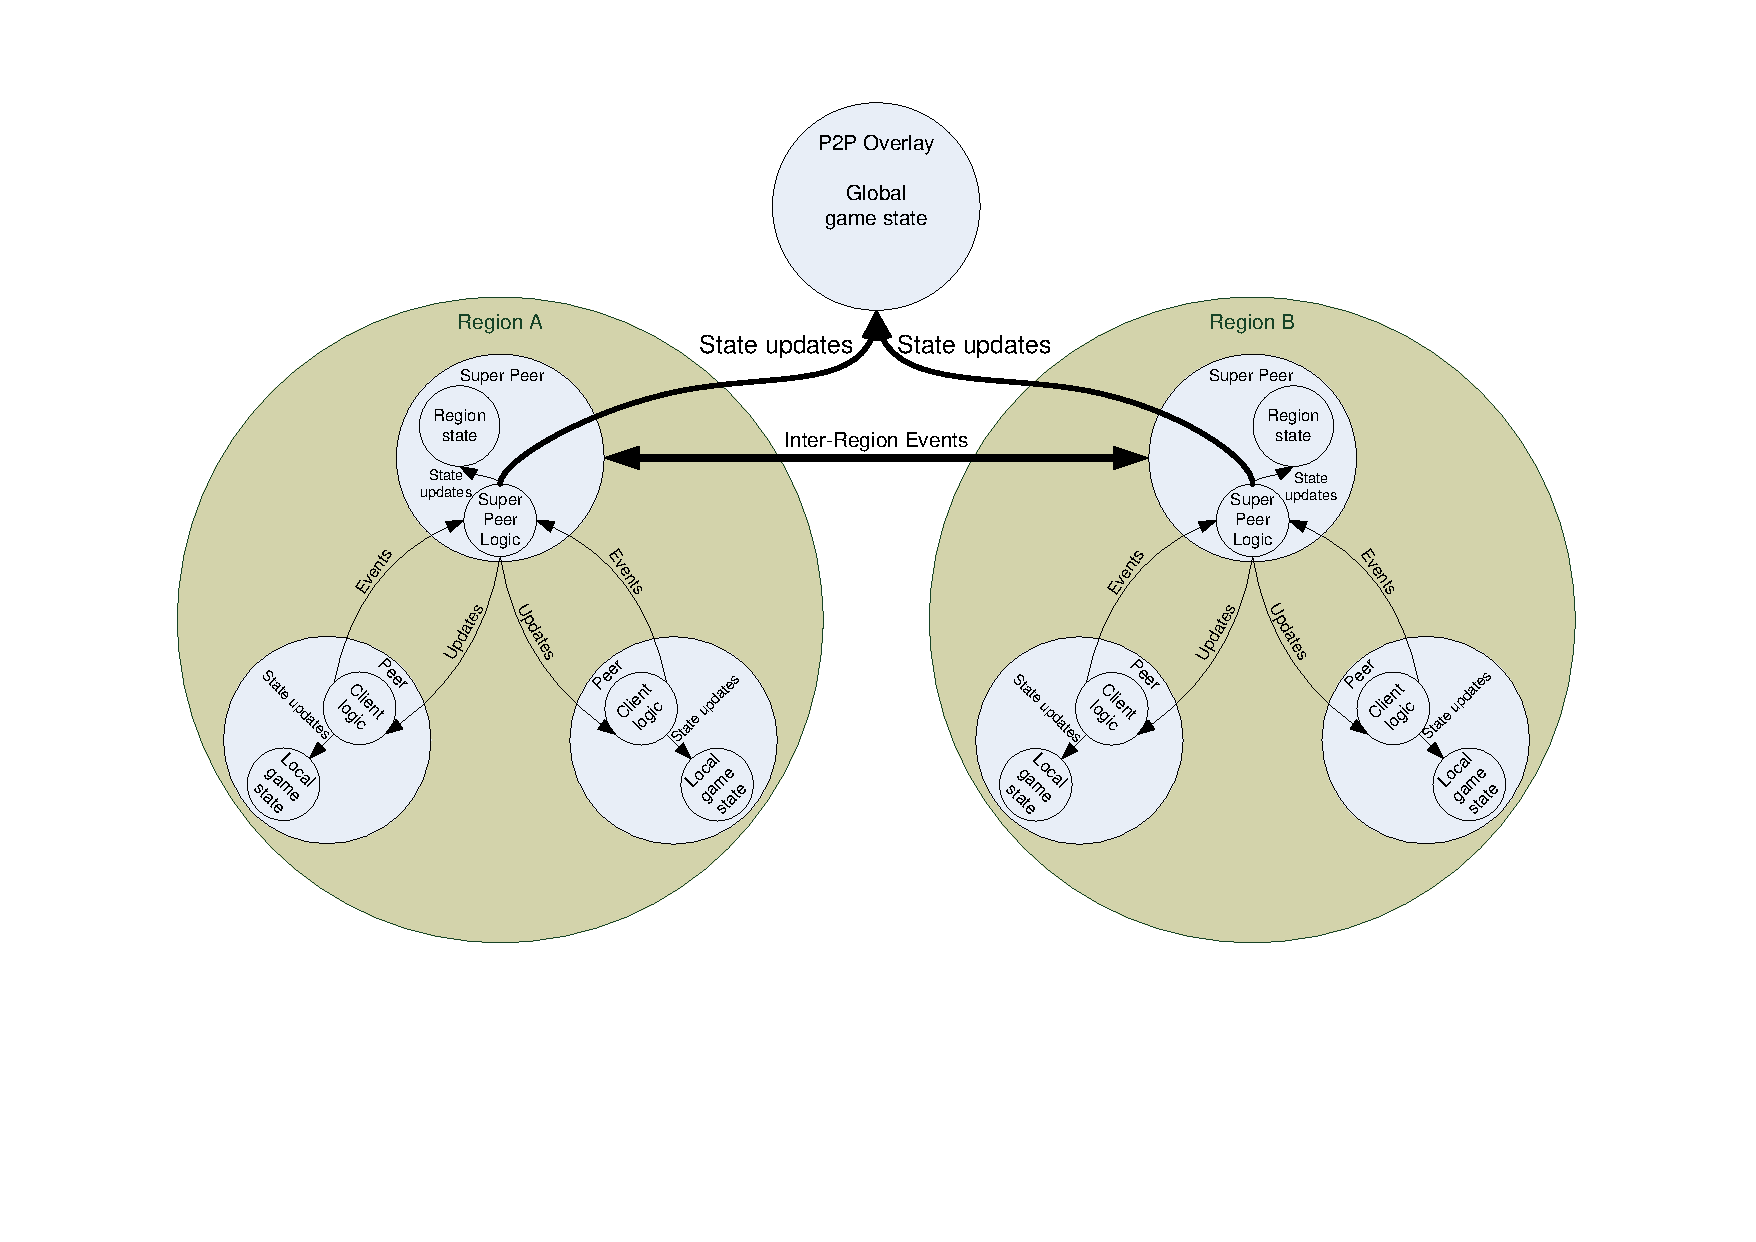
\includegraphics[clip=true, viewport=2cm 5cm 27cm 19.5cm, width=\textwidth]{region_based_CS_CM_P2PO}
 \caption{Hybrid region-based super peer storage with backup overlay storage consistency model}
 \label{fig_cs_region_o_cm}
\end{figure}
%
Figure \ref{fig_cs_region_o_cm} shows a type of Super Peer/Overlay hybrid storage implemented in  \cite{zoned_federation}. The model depicted in Figure \ref{fig_cs_region_o_cm} uses overlay storage, managed by regional super peers. The world is divided into regions, with each region controlled by a super peer. The complete region state is cached at every super peer, the same as with super peer storage. There also exists a backup
overlay storage architecture, to which data may be backed up for long term, redundant and secure storage. The hybrid region-based overlay storage contains many improvements over pure overlay storage as will be discussed in the following sections.

\subsubsection{Reliability}
\label{hybrid_storage_reliability}

Because of the use of overlay storage for backup, the hybrid region-based storage is almost as reliable as a pure overlay storage. It is classified as almost as reliable, because there is a delay between when data changes and when it is updated in the overlay. If a super peer fails during this time and the data was not backed-up to the overlay, that data could be lost. Backup super peers can, however, be implemented as described in Section
\ref{super_peer_storage_reliability} to improve the reliability of the hybrid storage model.

\subsubsection{Responsiveness}

Because all regional files are cached at super peers, the system is as responsive as super peer storage.

\subsubsection{Security}

Security in hybrid storage is still an issue, because of the inherent problems of the super peer storage model. Although it is more difficult for peers to access and manipulate data stored in the overlay, a malicious peer promoted to super peer status may manipulate the region data it controls.

It does seem possible to achieve higher levels of security, by checking data received from super peers, against the data stored in the overlay. Care should be taken with such a scheme, because the rate of change of data at the super peers might be higher than the rate that data are submitted to the overlay. Another issue is the time delay between data received from a super peer and data received from the overlay.

\subsubsection{Fairness}

The issue of fairness is also still present in hybrid storage. The system is fairer than super peer storage, since all peers share the load of the overlay storage, but there still exists the unfairness of the super peer storage. As all data exists in both the overlay storage as well as the super peer storage, the system is as unfair as super peer storage, because the same quantity of data as in super peer storage is not being distributed evenly amongst all peers.

\subsubsection{Existing architectures}

\begin{figure}[htbp]
 \centering
 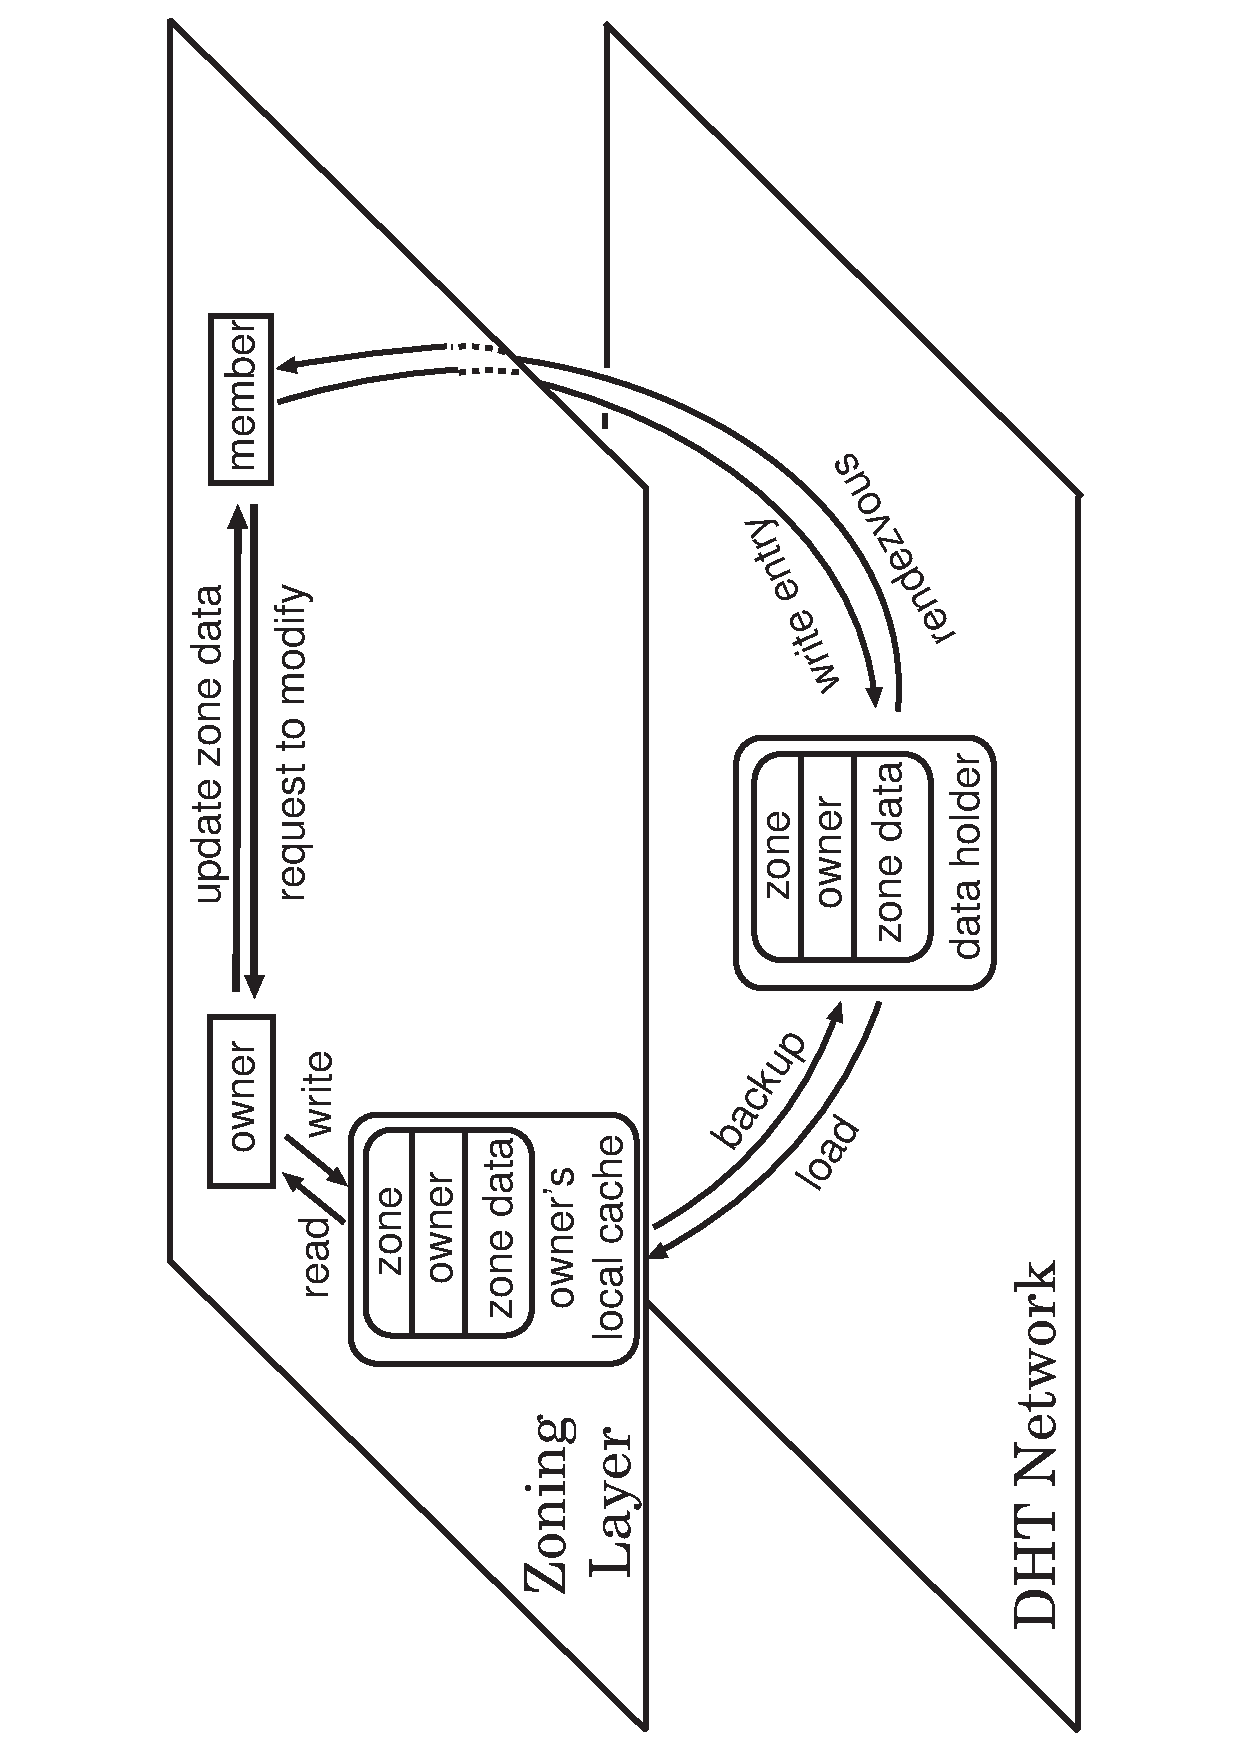
\includegraphics[clip=true, viewport=2cm 0cm 19cm 30cm, angle=-90, width=0.5\columnwidth]{zoned_federation_model}
 \caption{Zoned Federation Model \cite{zoned_federation}}
 \label{fig_zoned_federation_model}
\end{figure}
%
The first hybrid state persistency model for P2P MMVEs was proposed by Iimura et al. in 2004 \cite{zoned_federation} and called the ``Zoned Federation Model'', shown in Figure \ref{fig_zoned_federation_model}. The regional super peers are called ``Zone Owners'', which handle all events by clients in their zone or region. In the Zoned Federation model, a Zone Owner acts as the primary storage medium for all object states in the zone or region. As shown in Figure \ref{fig_cs_region_o_cm}, this is analogous to an update based model, divided into zones. The difference here is that the game state of all zone owners are regularly backed-up to overlay storage. The zoned federation model can thus be seen as a super peer/overlay storage hybrid. The super peers storage provides for low latency data storage and the overlay storage provides security and reliability.

An extended abstract, published by GauthierDickey et al. in 2004 \cite{hybrid_storage1}, proposed to distinguish between permanent and ephemeral data. Permanent data are described as data that should exist at all times and ephemeral data are described as data that need only exist for as long as its owner is in the game. An item, being dropped by a dispatched NPC, can be considered as ephemeral. When the peer on which the data is hosted leaves the area, that item can disappear. An example of permanent data is a player's inventory contents, which can further be classified as participatory data or a player's house, which can be classified as existential data. Participatory data are data that need only be available when a specific player is in the game and existential data are data that should be available, even when a certain player is not present in the game.

Categorising data by how long and under which circumstances the data should exist, may assist in the design of the storage model. Since ephemeral data does not have to exist after the player has left the game, it may be stored in primary memory. Participatory data might also be stored on the player's computer, but security issues will have to be kept in mind. Existential data will have to be stored somewhere other than on the player's computer, since other players will require the data, even in the absence of the player that might have left the game. GauthierDickey et al. did not explore how their data classification scheme might be translated into a state persistency model.

\subsection{Distance-based storage}
\label{distance_based_storage}

%Distance-based - overview
Distance based approaches, such as the Voronoi storage approaches \cite{Buyukkaya_voronoi_state_management}, \cite{Hu_voronoi_IM} and some more general approaches \cite{colyseus_distance_based}, \cite{solipsis}, store object data on the peer closest to the object in the virtual world. Some distance metric is used to determine on which peer an object should be stored.

\subsubsection{Responsiveness}

%Distance-based - issues
An issue with the above reasoning is that multiple peers are usually interacting with a single object. The examples of the NPC monster and trader are again relevant. Usually many players interact with a trader NPC and usually players attack monster NPCs in groups.

Multiple player interactions are, however, not as big an issue as others have suggested \cite{Fan_deisgn_issues_p2p}. In the best case, the object being used by a player is also hosted on that player's peer. If another player requires use of a remotely hosted object, that player may still interact with the object, where the host peer is simply acting as a server to that player. This essentially means that every player hosting an object becomes a server for that object. In the case where a player interacts with an object hosted locally, there is no object latency. In the case where a player
accesses a remotely hosted object, there is only one hop latency, the same as with a C/S or super peer application.

Issues with this approach stem from the fact the players are constantly moving. When players move, the objects in their regions change. Authoritative objects, therefore, have to be constantly transferred from one peer to another, which might cause significant network traffic. An object in transit might also delay interaction with that object. Because object transfer introduces overhead into the system, how regularly an object has to be transferred and whether the number of transferrals produce sufficiently low overhead to implement a real-time game, still have to be investigated.

Voronoi-based storage schemes also become unresponsive when communications are no longer between neighbours, but between two arbitrary peers in the
Voronoi overlay. When such communications occur, the average required time to route a message is $\OO{N^{1/2}}$ for a two-dimensional configuration.
Advancements have been made that suggest augmenting the Voronoi overlay with additional links to far off peers to create a small world network. This
reduces the average routing time to $\OO{\log{(N)}}$, the same as for overlay storage \cite{Steiner_voronoi_shortcuts}.

\subsubsection{Reliability}

Reliability, because of network churn, is still an issue. Peers will leave the network whenever a player stops playing the game, which makes it a common occurrence. When peers leave the network, the objects that are stored on that peer should still be accessible to other players. This will require transferring all objects contained in the leaving peer to another object, still present in the network. No literature could be found that dealt with the issue of reliability in a distance-based storage network.

The same solution that is used for overlay storage, namely the presence of redundant peers, might also be implemented for distance storage. Another structured overlay might be used to implement this redundancy in exactly the same way it is done with hybrid storage (mentioned in Section \ref{hybrid_storage_reliability}).

\subsubsection{Security}
\label{distance_based_storage_security}

The main issue with the distance based scheme is security. Peers that have the most interest in an object also have the most interest to manipulate that object in ways inconsistent with the game rules. When objects are hosted on peers that have the most interest in them, there will be a strong temptation to try and manipulate these objects. Because these modification are all local, it is also not possible to log the alterations and detect cheating. Means by which local objects can be secured have to be found or distance based algorithms with quorum need to be investigated.

This security issue is similar to that of super peer storage, in that local data can be accessed, thus circumventing the certification system. With this circumvention, the objectives of authentication, authorisation, confidentiality, trust, privacy and identity management are all compromised.

\subsubsection{Fairness}

Distance-based storage is relatively fair as all objects are distributed amongst all peers. Where the system becomes somewhat unfair is when a peer is nearest to a large number of objects. For Voronoi regioning approaches, this is when a peer's Voronoi region contains many more objects than the average number of objects hosted by other peers. This might not be a major issue, depending on how long the objects have to be hosted on the overloaded peer. This will depend on the movement of the overloaded peer as well as that of neighbouring peers. The use of aggregators as a proposed solution to this problem is discussed in Section \ref{distance_based_existing_archs}.

\subsubsection{Existing architectures}
\label{distance_based_existing_archs}

%Colyseus, 2006
Bharambe et al. created the Colyseus architecture in 2006 \cite{colyseus_distance_based}. The architecture is designed to support First Person Shooter (FPS) games and implemented to function with Quake II. Mutable game objects are stored on the peer that is nearest to the object in the game world. An ``object placer'' component is mentioned, but the details of the placement algorithm are left for future work. The architecture also does not implement non-volatile state persistency, since this is not required for normal FPS games, where object states need only exist to the end of a
round and where players generally do not leave before the end of the round. This means that object states are only stored in primary memory, until the end of a game round.

%Solipsis, 2008
The Solipsis architecture was created by Frey et al. in 2008 \cite{solipsis}. The architecture uses Voronoi diagrams to create virtual regions. Stationary objects are maintained by site peers until a player picks up an object. When an object is picked up, control of that object is transferred to the player that picked up the object. The Solipsis architecture focusses on distributed physics computation and when a player gains control of an object, that player is responsible for the object's physics computations. That player should also save all object state until a new player takes the object, at which time control is transferred to her. Control can also be transferred back to a site peer if an object remains stationary for some
time.

What differentiates the Solipsis distance-based storage from the other architectures presented in this section, is that object states are only handled by peers as long as those peers directly use an object. At other times, those objects are handled by site peers. This differs from other distance-based storage techniques, where all objects that are nearest to a player in the virtual world are controlled by that player.

%Buyukkaya and Abdallah, 2008 and Hu et al., 2008
In 2008, papers were published by Buyukkaya and Abdallah \cite{Buyukkaya_voronoi_state_management}, and Hu et al. \cite{Hu_voronoi_IM}, proposing to use Voronoi diagrams \cite{voronoi_diagrams_survey} to implement distance-based storage. Voronoi state management schemes host the mutable objects on the peer in which region the object exists. As peers move around in the virtual world, the Voronoi diagram has to be constantly recalculated and objects have to be moved to new owner peers as the regions in which they fall change. The significant advantage of the Voronoi approach is that peers only require connections with their neighbours, and peers within their AoI.

\begin{figure}[htbp]
 \centering
 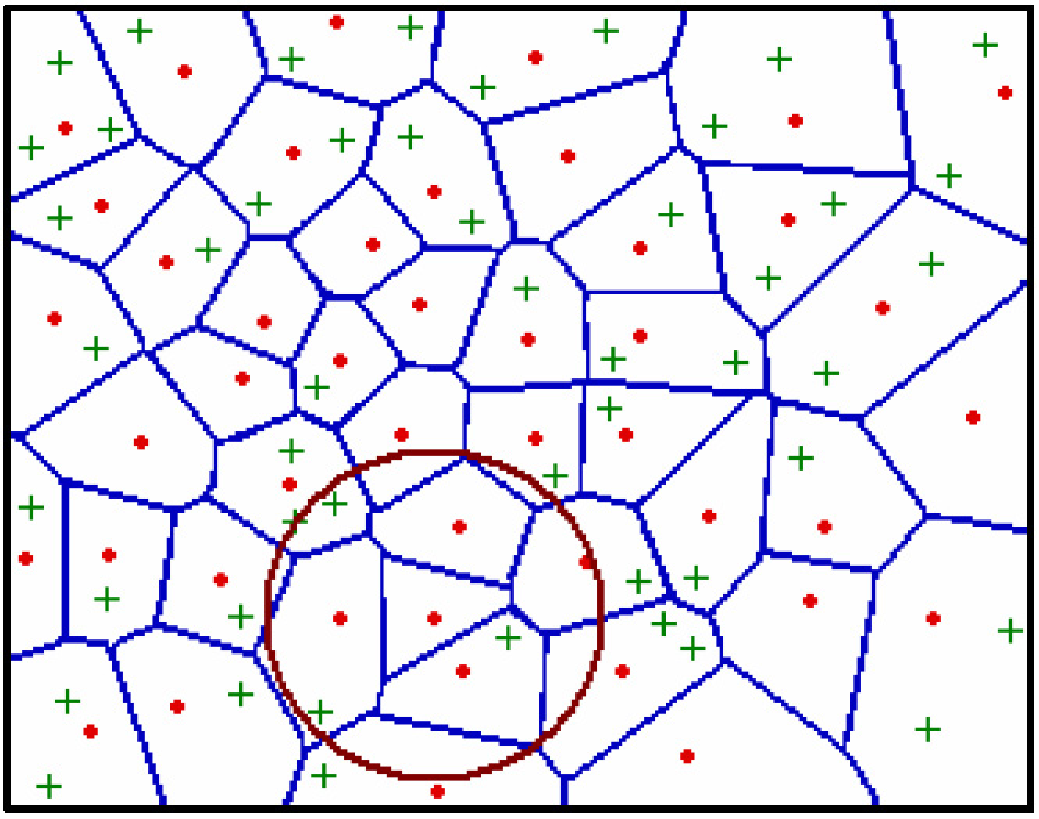
\includegraphics[width=0.4\columnwidth]{voronoi_diagram}
 \caption{Voronoi Diagram \cite{Buyukkaya_voronoi_state_management}}
 \label{fig_voronoi_diagram}
\end{figure}
%
Voronoi storage approaches use Voronoi diagrams to determine on which peers objects should be stored. Given a set of points, the Voronoi diagram of the set of points is the partition of the plane, which associates a region around every point in such a way that all other points contained in the region are closer to the centre point than any other point in the set. Figure \ref{fig_voronoi_diagram} shows a Voronoi diagram, where the lines define the region boundaries, the dots define the players, which make up the set of points for which the diagram was calculated, the plus signs represent mutable objects and the circle represents the AoI of a central point in the set.

For the Voronoi approaches a peer controls and hosts all objects within its Voronoi region. The reasoning is that there is a high probability that the player closest to the object is also the player using the object. Examples of this are where a player is trading or fighting with an NPC.

A thesis by Chang also describes the Voronoi approach in more detail and how to achieve game state consistency amongst all peers in a Voronoi network \cite{Chang_Voronoi_state_management_masters}. What distinguishes this work from the others is the implementation of a load balancing mechanism. When peers get overloaded, another, more powerful peer is chosen as an Aggregator. The Aggregator assumes responsibility for a larger area that encompasses multiple peers. This scheme will reduce the load on peers with minimal resources, but it is uncertain how this would reduce load when peers with an average number of resources in an area become overloaded.

The works by Buyukkaya and Abdallah, Hu et al., and Chang form part of the VAST project, which is being created to be a fully functional P2P overlay architecture, using Voronoi diagrams as its basis \cite{VAST}. The reason why state persistency in Voronoi-based P2P MMVEs architectures are mostly distance-based approaches, is because the Voronoi diagram immediately identifies which objects are closest to a particular peer, and therefore, which objects that peer has to host. Architectures not making use of Voronoi diagrams still require some other mechanism to allocate object hosting to peers.

\section{Conclusion}

After providing an overview of the classic C/S and C/MS state persistency techniques, the chapter classified P2P MMVE state persistency techniques into super peer based, overlay based, distance based and hybrid storage. The advantages and disadvantages of each method were discussed after identifying key challenges that state persistency techniques have to solve. These challenges are: fairness, overhead, reliability, responsiveness, scalability and security.

Supper peer storage can be seen as a C/S type storage implementation, where every region has a super peer that stores all data for that region. Overlay storage is a fully distributed, P2P approach to storage, where every peer stores data as part of a P2P overlay network. Hybrid region based storage combines super peer and overlay storage to improve the overall storage performance. Distance based storage is a different paradigm that stores game objects on the nearest peer to that game object. This type of storage is usually characterised by the use of Voronoi diagrams to
determine which peers are nearest to which objects.

Super peer storage is characterised by its high level of responsiveness and ease of implementation. Overlay storage is characterised by its high level of fairness and reliability. Hybrid region-based storage combines the two previous schemes and has high levels of reliability and responsiveness. Distance based storage is also very responsive and can be made both reliable and fair.

Security is still an issue for all storage types. Super peer storage has the issues that are usually present in a centralised system, namely low fairness, security and also not being reliable and not resistant to failure. The main issue with overlay storage is its unresponsiveness, because of the routing delay in the P2P overlay. Hybrid storage suffers from the disadvantages of super peer storage, namely low fairness and security, due to all files still stored on super peers. The main issue of distance based storage is security, because players that have the most incentive to alter object states own those objects.

Distance based storage is still fairly immature, but shows a lot of promise. No publicly available implementation could be found for this type of storage. Where this type of storage was used, it was explained as distance based storage, but most of the details were left out. Distance-based storage holds the most promise to fulfill all P2P MMVE requirements.

We conclude that there exists no single state persistency architecture, currently in use, that is suited to P2P MMVEs. None of the storage techniques reviewed meet the requirements of a real-time distributed application, such as an MMVE. What is required is a state persistency architecture, specifically geared towards data persistency in P2P MMVEs, that meet all the challenges of the application.

To compensate for the deficiencies of the existing architecture, we combine overlay storage, distance-based storage and to some degree, super peer storage to propose a hybrid architecture, which meets all storage requirements. The design of this novel architecture, called Pithos, is discussed in the next chapter.
